%%%%%%%%%%%%%%%%%%%%%%%%%%%%%%%%%%%%%%%%%%%%%%%%%%%%%%%%%%%%%%%%%%%%%
% LaTeX Template: Project Titlepage Modified (v 0.1) by rcx
%
% Original Source: http://www.howtotex.com
% Date: February 2014
% 
% This is a title page template which be used for articles & reports.
% 
% This is the modified version of the original Latex template from
% aforementioned website.
% 
%%%%%%%%%%%%%%%%%%%%%%%%%%%%%%%%%%%%%%%%%%%%%%%%%%%%%%%%%%%%%%%%%%%%%%
\documentclass[12pt]{report}
\usepackage[a4paper]{geometry}
\usepackage[myheadings]{fullpage}
\usepackage{fancyhdr}
\usepackage{lastpage}
\usepackage{graphicx, wrapfig, subcaption, setspace, booktabs}
\usepackage[english]{babel}
\usepackage{color}
\usepackage{hyperref}
\usepackage{array}
\usepackage{supertabular}
\usepackage{hhline}
\usepackage{enumitem}
\usepackage[T1]{fontenc}
\usepackage[utf8]{inputenc}
\usepackage{graphicx}
\newcommand{\HRule}[1]{\rule{\linewidth}{#1}}
\renewcommand{\theenumii}{\arabic{enumii}.}
\addto\captionsenglish{
  \renewcommand{\contentsname}
    {Innhold}
}
\onehalfspacing
\setcounter{tocdepth}{5}
\setcounter{secnumdepth}{5}
%-------------------------------------------------------------------------------
% HEADER & FOOTER
%-------------------------------------------------------------------------------
\pagestyle{fancy}
\fancyhf{}
\setlength\headheight{15pt}
\fancyhead[L]{Team D} 
\fancyhead[R]{Universitetet i Bergen}
\fancyfoot[R]{Page \thepage\ of \pageref{LastPage}}
%-------------------------------------------------------------------------------
% TITLE PAGE
%-------------------------------------------------------------------------------
\begin{document}
\title{ \normalsize \textsc{}
		\\ [2.0cm]
		\HRule{0.5pt} \\
		\LARGE \textbf{\uppercase{TD Uteliv }}
		\HRule{2pt} \\ [0.5cm]
		\normalsize \today \vspace*{5\baselineskip}}
\date{}
\author{
		Team D  \\ 
		Universitetet i Bergen \\
		Informatikk }
\maketitle
\tableofcontents
\newpage
%-------------------------------------------------------------------------------
% BODY
%-------------------------------------------------------------------------------
\section*{Bruksm{\o}nstertekst:}
\addcontentsline{toc}{section}{Bruksm{\o}nstertekst:}
\textbf{Tittel}: Eliminere motstanderne
\bigskip \\
\textbf{Akt{\o}rer}: Spiller, System
\bigskip \\
\textbf{Prim{\ae}rakt{\o}r}: Spiller
\bigskip \\
\textbf{Tid}: 45 sekunder før fiender genereres, runden varer frem til alle fiendene er av brettet eller en fiende overlever siste utested 
\bigskip \\
\textbf{M{\aa}l}: Skyte flasker og lignende på alle motstandere slik at de dør
\bigskip \\
\textbf{Pre-conditions:} Spillet er startet p{\aa} en datamaskin
\subsubsection*{Hovedflyt:}
\begin{enumerate}
\item Systemet viser hovedmeny
\item Spiller velger å starte spillet
\item Systemet genererer bane
\item Spiller kan velge sette ut tårn og oppgradere dem
\item Spiller prøver å sette ut tårn
\item Systemet beregner om spiller har råd til å sette ut tårn
\item Systemet plasserer tårn der spiller ønsker
\item Spiller oppgraderer tårn
\item Systemet beregner om spiller har råd til å oppgradere tårn
\item Systemet oppgraderer tårn
\item Spiller velger å starte runden (slik at fiendene kommer)
\item Systemet genererer fiender som prøver å komme seg til målet
\item Systemet beregner skaden til fiende(ne) utgjort av de forskjellige tårnenes våpen
\item Systemet beregner fiendens helse om fiende ble truffet
\item Systemet eliminerer fiender med helse mindre enn 1
\item Spillers tårn har drept alle fiendene
\item Spiller har vunnet runden
\item Systemet forteller spiller at spiller har vunnet runden
\end{enumerate}
\textit{Steg 4-16 går i loop til x antall runder er vunnet}
\begin{enumerate}[resume]
\item Spiller har vunnet x antall runder
\item Systemet forteller at spiller har vunnet alle rundene
\item Systemet viset hovedmeny
\end{enumerate}
\subsubsection*{Alternative handlinger:}
\begin{enumerate}[label=\Alph*]
\item
\bigskip
\begin{enumerate}
\item @1 Spiller velger å avslutte spillet
\item Systemet avslutter spillet
\end{enumerate}

\item
\bigskip
\begin{enumerate}
\item @2 Spiller velger å pause spillet
\item Systemet pauser spillet
\item Systemet viser pausemeny
\end{enumerate}

\item
\bigskip
\begin{enumerate}
\item @6 Systemet beregner at spiller ikke har råd til å sette ut tårn
\item Systemet setter ikke ut tårn
\item Gjenoppta @4
\end{enumerate}

\bigskip
\begin{enumerate}
\item @9 Systemet beregner at spiller ikke har råd til å oppgradere tårn
\item Systemet oppgraderer ikke tårn
\item Gjenoppta @4
\end{enumerate}

\item 
\bigskip
\begin{enumerate}
\item @16 En eller flere fiender overlever
\item Spiller har tapt spillet
\item Systemet forteller at spiller har tapt spillet
\item Gjenoppta @1
\end{enumerate}
\end{enumerate}

\section*{Bruksm{\o}nsterdiagram:}
\addcontentsline{toc}{section}{Bruksm{\o}nsterdiagram:}
\vspace{1cm}
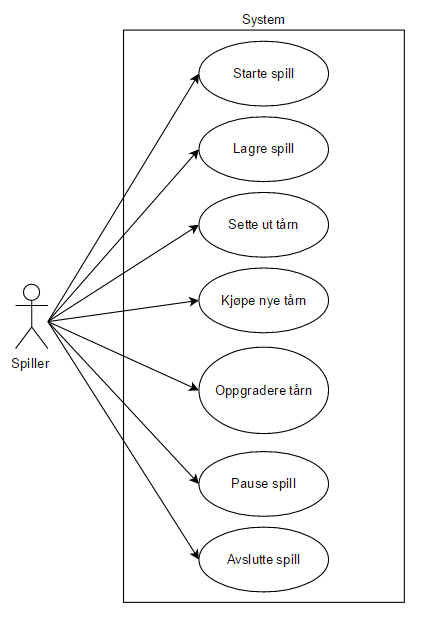
\includegraphics{use_case_diagram_t.png}
\end{document}